\chapter{Konsentrasi dan Pengenceran}\label{ch:g10:concentration-and-dilution}

Sebuah kantong infus tergantung di atas tempat tidur pasien. Labelnya
berbunyi ``natrium klorida 0.9 \%'': garam dalam air, tidak lebih.
Namun angka 0.9 itu bukan perkara kecil. Terlalu sedikit garam, dan
sel-sel darah pasien akan menggembung oleh air; terlalu banyak, dan
sel-sel itu akan mengerut. Sebuah larutan tidak cukup diuraikan dengan
bahan-bahannya saja, tetapi dengan berapa banyak \omterm{def:g6:solutions-and-solubility:solute}{zat terlarut} yang
dikandung setiap volumenya, yaitu konsentrasinya. Bab ini mengukur
konsentrasi, menyiapkan larutan dengan konsentrasi yang tepat, dan
mengencerkannya.

\begin{recall}
Larutan tersusun atas \omterm{def:g6:solutions-and-solubility:solute}{pelarut} dan satu \omterm{def:g6:solutions-and-solubility:solute}{zat terlarut} atau lebih;
\omterm{def:g6:solutions-and-solubility:solubility}{kelarutan} adalah massa \omterm{def:g6:solutions-and-solubility:solute}{zat terlarut} terbesar yang dapat dilarutkan oleh
sejumlah tertentu \omterm{def:g6:solutions-and-solubility:solute}{pelarut} (\cref{ch:g6:solutions-and-solubility}).
\omterm{def:g10:the-mole:amount}{Jumlah zat} sebuah spesies adalah $n = m/M$, dalam \omterm{def:g10:the-mole:amount}{mol}
(\cref{ch:g10:the-mole}).
\end{recall}

\begin{omfigure}
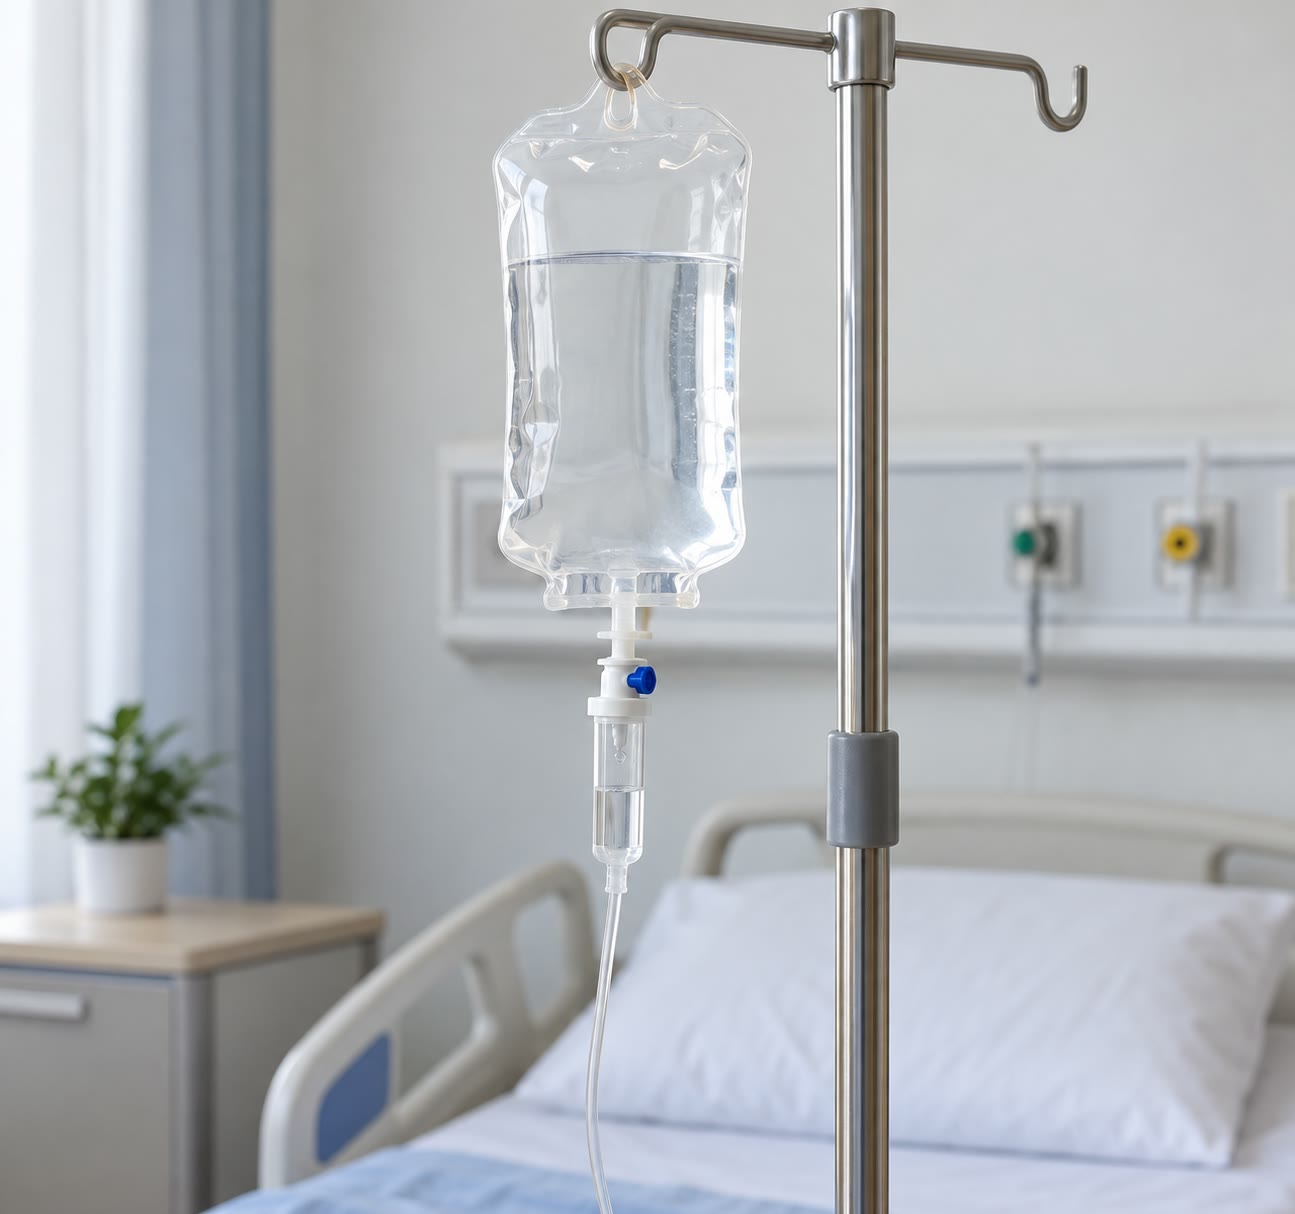
\includegraphics[width=0.42\linewidth]{images/book1/ai/g10-drip-bag.jpg}

{\small Sekantong infus larutan garam: konsentrasinya harus tepat.}
\end{omfigure}

\section{Konsentrasi massa}

\begin{definition}[Konsentrasi massa]\label{def:g10:concentration-and-dilution:mass-concentration}
Yang disebut \emph{konsentrasi massa}\index{konsentrasi massa} $C_m$
sebuah \omterm{def:g6:solutions-and-solubility:solute}{zat terlarut} dalam larutan adalah massa \omterm{def:g6:solutions-and-solubility:solute}{zat terlarut} yang \omterm{def:g2:mixing-and-dissolving:dissolve}{larut}
per volume larutan:
\[
  C_m = \frac{m_{\text{zat terlarut}}}{V_{\text{larutan}}},
\]
dalam gram per liter (\si{g/L}).
\end{definition}

\begin{example}[Air gula]\label{ex:g10:concentration-and-dilution:sugar}
Sebanyak \qty{20}{g} gula dilarutkan dalam air, dan larutannya
dicukupkan sampai \qty{0.50}{L}. \omterm{def:g10:concentration-and-dilution:mass-concentration}{Konsentrasi massa} gulanya adalah
$C_m = \qty{20}{g} / \qty{0.50}{L} = \qty{40}{g/L}$. Setiap bagian
larutan itu memiliki konsentrasi yang sama: segelas larutan itu
sebanyak \qty{0.20}{L} memuat
$\qty{40}{g/L} \times \qty{0.20}{L} = \qty{8.0}{g}$ gula.
\end{example}


\begin{remark}[Volumenya adalah volume larutan]\label{rem:g10:concentration-and-dilution:volume}
Volume dalam $C_m$ adalah volume seluruh larutan, bukan volume air yang
dituangkan: melarutkan \omterm{def:g6:solutions-and-solubility:solute}{zat terlarut} sedikit mengubah volume. Itulah
sebabnya sebuah larutan selalu \emph{dicukupkan} sampai volume akhir
yang diketahui, di dalam labu yang diberi tanda untuk volume itu.
\end{remark}

\begin{remark}[Konsentrasi bukan kelarutan]\label{rem:g10:concentration-and-dilution:not-solubility}
% ledger: sol:NaCl, saline:NaCl
\omterm{def:g6:solutions-and-solubility:solubility}{Kelarutan} sebuah \omterm{def:g6:solutions-and-solubility:solute}{zat terlarut} adalah konsentrasi \emph{terbesar} yang
dapat dicapainya; sebuah larutan dapat memiliki konsentrasi berapa pun
dari nol sampai batas itu. Natrium klorida \omterm{def:g2:mixing-and-dissolving:dissolve}{larut} sampai sekitar
\qty{360}{g} per kilogram air pada \qty{25}{\celsius}; kantong infus
hanya memuat \qty{9}{g} per liter, sangat jauh dari jenuh.
\end{remark}

\begin{remark}[Persentase pada label]\label{rem:g10:concentration-and-dilution:percent}
% ledger: saline:NaCl
Pada label obat dan makanan, ``0.9 \%'' untuk padatan yang \omterm{def:g2:mixing-and-dissolving:dissolve}{larut} dalam
air biasanya berarti \qty{0.9}{g} \omterm{def:g6:solutions-and-solubility:solute}{zat terlarut} per \qty{100}{mL}
larutan. Dalam gram per liter nilainya sepuluh kali lebih besar: kantong
infus itu memuat \qty{9.0}{g/L} natrium klorida.
\end{remark}

\section{Konsentrasi molar}

\begin{definition}[Konsentrasi molar]\label{def:g10:concentration-and-dilution:molar-concentration}
Yang disebut \emph{konsentrasi molar}\index{konsentrasi molar} $c$
sebuah \omterm{def:g6:solutions-and-solubility:solute}{zat terlarut} dalam larutan adalah jumlah \omterm{def:g6:solutions-and-solubility:solute}{zat terlarut} yang \omterm{def:g2:mixing-and-dissolving:dissolve}{larut}
per volume larutan:
\[
  c = \frac{n_{\text{zat terlarut}}}{V_{\text{larutan}}},
\]
dalam \omterm{def:g10:the-mole:amount}{mol} per liter (\si{mol/L}).
\end{definition}

\begin{proposition}[Dari konsentrasi yang satu ke yang lain]\label{prop:g10:concentration-and-dilution:link}
Untuk \omterm{def:g6:solutions-and-solubility:solute}{zat terlarut} bermassa molar $M$,
\[
  C_m = c \times M .
\]
\end{proposition}

\begin{proof}
$C_m = m / V = (n \times M) / V = (n / V) \times M = c \times M$.
\end{proof}

\begin{example}[Kantong infus dalam mol]\label{ex:g10:concentration-and-dilution:drip}
% ledger: saline:NaCl, saline:Na, aw:Na, aw:Cl
Kantong infus memuat \qty{9.0}{g/L} natrium klorida, yang \omterm{def:g10:the-mole:molar-mass}{massa
molarnya} \qty{58.5}{g/mol}. \omterm{def:g10:concentration-and-dilution:molar-concentration}{Konsentrasi molarnya} adalah
\[
  c = \frac{C_m}{M} = \frac{\qty{9.0}{g/L}}{\qty{58.5}{g/mol}}
    = \qty{0.154}{mol/L}.
\]
Label dari pabriknya memberikan angka yang sama dari arah sebaliknya:
154 perseribu \omterm{def:g10:the-mole:amount}{mol} \omterm{def:g9:ions:ion}{ion} natrium per liter.
\end{example}

\begin{remark}[Ion dalam larutan]\label{rem:g10:concentration-and-dilution:ions}
Natrium klorida \omterm{def:g2:mixing-and-dissolving:dissolve}{larut} sebagai \omterm{def:g9:ions:ion}{ion-ion} terpisah \ce{Na+} dan \ce{Cl-}
(\cref{ch:g9:ions}): larutan natrium klorida \qty{0.154}{mol/L} memuat
\qty{0.154}{mol/L} \omterm{def:g9:ions:ion}{ion} natrium dan \qty{0.154}{mol/L} \omterm{def:g9:ions:ion}{ion} klorida.
Bagaimana sebuah padatan \omterm{def:g9:ions:ion}{ion} terurai di dalam air menjadi pokok bahasan
sebuah bab berikutnya.
\end{remark}

\begin{omfigure}
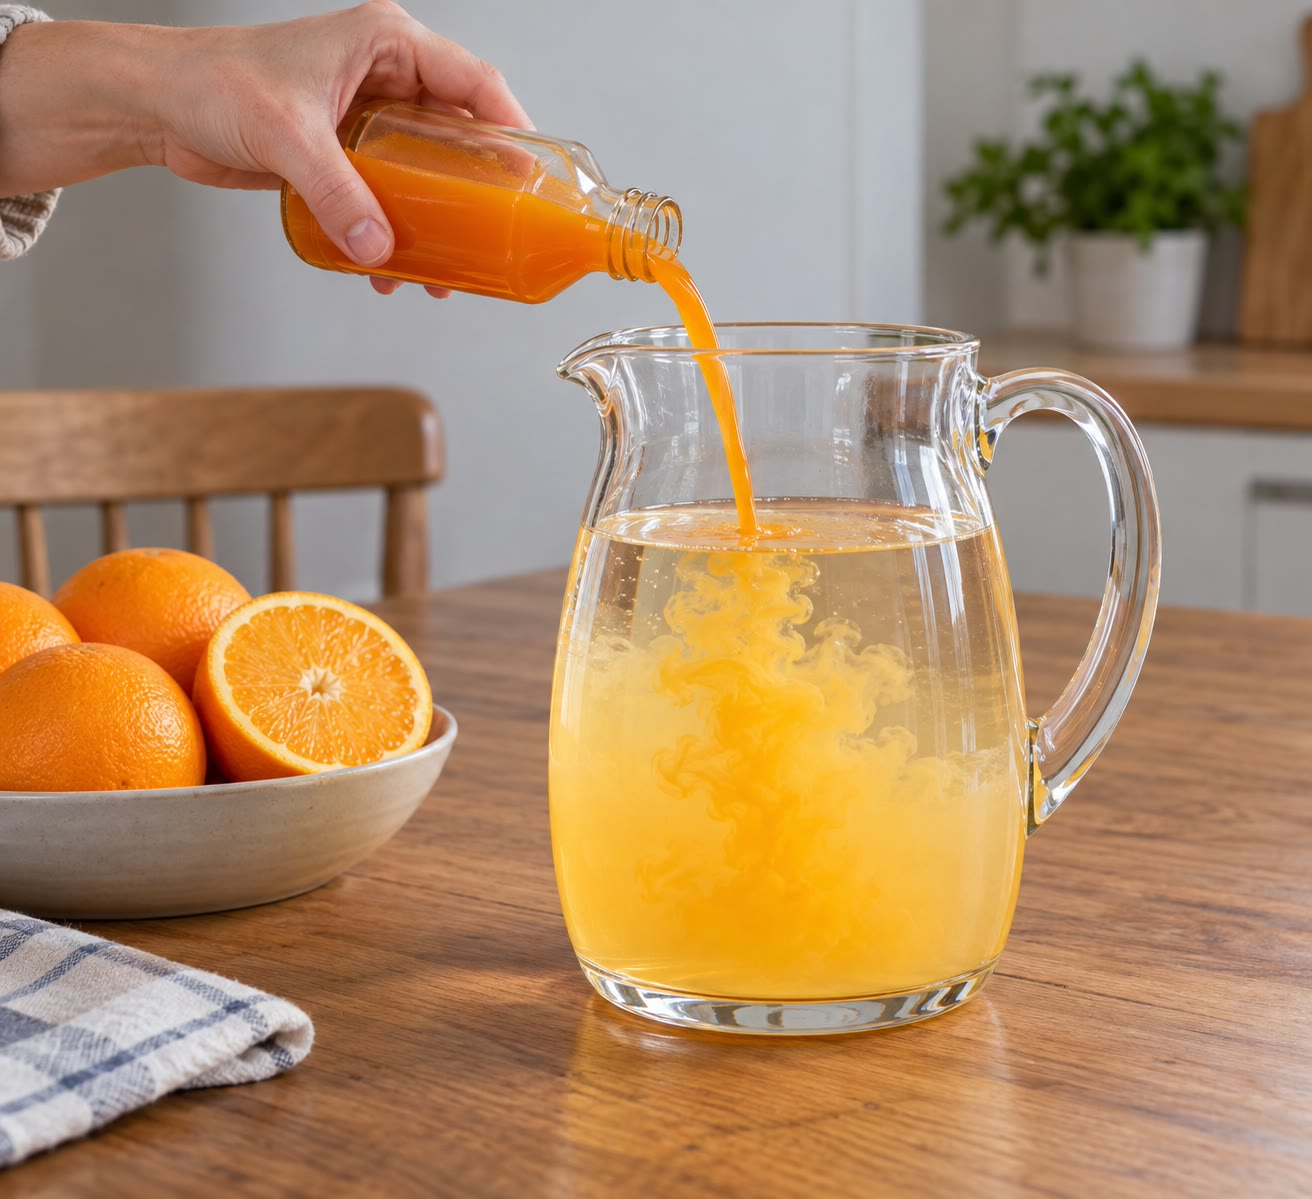
\includegraphics[width=0.45\linewidth]{images/book1/ai/g10-squash-jug.jpg}

{\small Sirop dari botol diencerkan dengan air di dalam teko: minuman itu
memuat jumlah sirop buah yang sama, dalam volume yang lebih besar.}
\end{omfigure}

\section{Menyiapkan larutan dengan melarutkan}

\begin{method}[Menyiapkan larutan dengan melarutkan padatan]\label{met:g10:concentration-and-dilution:dissolving}
Untuk menyiapkan larutan bervolume $V$ dengan \omterm{def:g10:concentration-and-dilution:molar-concentration}{konsentrasi molar} $c$:
\begin{enumerate}
  \item Hitung \omterm{def:g10:the-mole:amount}{jumlah zat} yang diperlukan, $n = c \times V$, dan massa
        yang harus ditimbang, $m = n \times M$.
  \item Timbang padatan sebanyak massa ini di dalam cawan kecil di atas
        neraca.
  \item Tuang padatan itu melalui corong ke dalam labu ukur bervolume
        $V$; bilas cawan dan corong dengan air suling ke dalam labu,
        agar tidak ada padatan yang hilang.
  \item Tambahkan air suling sampai sekitar setengah labu dan goyangkan
        sampai semua padatan \omterm{def:g2:mixing-and-dissolving:dissolve}{larut}.
  \item Tambahkan air suling sampai tanda batas, tetes-tetes terakhir
        dengan pipet tetes; sumbat labunya dan bolak-balikkan beberapa
        kali untuk \omterm{def:g2:mixing-and-dissolving:mix}{mencampur}.
\end{enumerate}
\end{method}

\begin{omfigure}
\begin{tikzpicture}[font=\small, scale=1.05]
  % 1. weigh
  \pic[transform shape] at (0,0) {balance};
  \fill[black!8, draw=black!55] (-0.45,0.8) -- (0.45,0.8) -- (0.38,0.98)
    -- (-0.38,0.98) -- cycle;
  \fill[white, draw=black!40] (-0.25,0.98) .. controls (-0.1,1.15) and
    (0.1,1.15) .. (0.25,0.98) -- cycle;
  \node[align=center, anchor=north] at (0,-0.2) {1. timbang\\ padatannya};
  % 2. transfer through a funnel
  \pic[transform shape] at (3.2,0) {volflask={0.08}{omWater}};
  \pic[transform shape] at (3.2,3.0) {funnel};
  \draw[omProp, thick, -{Stealth}] (2.4,5.0) -- (2.85,4.65);
  \node[align=center, anchor=north] at (3.2,-0.2) {2. pindahkan,\\ bilas ke dalam};
  % 3. half full, swirl
  \pic[transform shape] at (6.4,0) {volflask={0.45}{omWater}};
  \draw[omProp, thick, -{Stealth}] (5.55,0.5) arc[start angle=200,
    end angle=340, x radius=0.9, y radius=0.3];
  \node[align=center, anchor=north] at (6.4,-0.2) {3. setengah penuh:\\ goyang hingga larut};
  % 4. to the mark
  \pic[transform shape] at (9.6,0) {volflask={1}{omWater}};
  \fill[black!45] (9.43,3.6) rectangle (9.77,3.85);
  \draw[omDef, thick, <-] (9.82,2.9) -- (10.6,3.3) node[right] {tanda batas};
  \node[align=center, anchor=north] at (9.6,-0.2) {4. isi sampai tanda,\\
    sumbat, campur};
\end{tikzpicture}

{\small Menyiapkan larutan dengan melarutkan padatan: timbang, pindahkan,
larutkan, lalu cukupkan sampai tanda batas labu ukur.}
\end{omfigure}

\begin{inthelab}[Mengisi sampai tanda batas]
Tanda batas sebuah labu ukur adalah sebuah cincin di sekeliling
lehernya. Air di dalam tabung kaca yang sempit tidak berakhir datar:
permukaannya melengkung ke bawah di bagian tengah, membentuk meniskus.
Labu itu penuh ketika \emph{dasar} meniskus menyentuh tanda batas, dilihat
dengan mata sejajar tanda itu, sehingga bagian depan dan bagian belakang
cincin itu tampak sebagai satu garis. Jika dilihat dari atas atau dari
bawah, tinggi permukaan dapat tampak benar padahal tidak.
\end{inthelab}

\begin{omfigure}
\begin{tikzpicture}[font=\small]
  \newcommand{\neck}[2]{% x, meniscus bottom height
    \fill[omWater] (#1-0.5,0) -- (#1-0.5,{#2+0.25}) .. controls
      (#1-0.25,#2) and (#1+0.25,#2) .. (#1+0.5,{#2+0.25}) -- (#1+0.5,0) -- cycle;
    \draw[black!60, line width=0.8pt] (#1-0.5,0) -- (#1-0.5,3);
    \draw[black!60, line width=0.8pt] (#1+0.5,0) -- (#1+0.5,3);
    \draw[omDef, line width=0.9pt] (#1-0.5,1.5) -- (#1+0.5,1.5);
    \draw[black!50] (#1-0.5,{#2+0.25}) .. controls (#1-0.25,#2) and
      (#1+0.25,#2) .. (#1+0.5,{#2+0.25});}
  \newcommand{\eye}[2]{% x, y: an eye looking to the right
    \draw[black!70] (#1-0.25,#2) .. controls (#1-0.1,#2+0.18) and
      (#1+0.1,#2+0.18) .. (#1+0.2,#2) .. controls (#1+0.1,#2-0.18) and
      (#1-0.1,#2-0.18) .. (#1-0.25,#2);
    \fill[black!70] (#1+0.05,#2) circle (0.06);}
  % right
  \neck{1.5}{1.5}
  \eye{-0.4}{1.5}
  \draw[dashed, black!50] (-0.1,1.5) -- (2.4,1.5);
  \node[align=center] at (1.5,-0.55) {benar: mata sejajar,\\ dasar di tanda};
  % too high
  \neck{6}{1.85}
  \eye{4.1}{1.85}
  \draw[dashed, black!50] (4.4,1.85) -- (6.9,1.85);
  \node[align=center] at (6,-0.55) {air terlalu banyak:\\ meniskus di atas};
  % too low
  \neck{10.5}{0.85}
  \eye{8.6}{0.85}
  \draw[dashed, black!50] (8.9,0.85) -- (11.4,0.85);
  \node[align=center] at (10.5,-0.55) {air terlalu sedikit:\\ meniskus di bawah};
\end{tikzpicture}

{\small Leher sebuah labu ukur, diperbesar dan dilihat dengan mata
sejajar meniskus. Garis biru adalah tanda batas. Hanya labu di sebelah
kiri yang terisi dengan benar.}
\end{omfigure}

\section{Mengencerkan}

\begin{definition}[Pengenceran, larutan induk, faktor pengenceran]\label{def:g10:concentration-and-dilution:dilution}
Sebuah \emph{pengenceran}\index{pengenceran} menurunkan konsentrasi
sebuah larutan dengan menambahkan \omterm{def:g6:solutions-and-solubility:solute}{pelarut}. Larutan pekat yang diambil
pada awalnya disebut \emph{larutan induk}\index{larutan induk}. Yang
disebut \emph{faktor pengenceran}\index{faktor pengenceran} $F$ adalah
perbandingan konsentrasi larutan induk terhadap konsentrasi larutan
encer:
\[
  F = \frac{c_{\text{induk}}}{c_{\text{encer}}} .
\]
\end{definition}

\begin{proposition}[Jumlah zat terlarut tetap]\label{prop:g10:concentration-and-dilution:kept}
Selama \omterm{def:g10:concentration-and-dilution:dilution}{pengenceran}, jumlah \omterm{def:g6:solutions-and-solubility:solute}{zat terlarut} tidak berubah: jika \omterm{def:g10:concentration-and-dilution:dilution}{larutan
induk} bervolume $V_0$ dengan konsentrasi $c_0$ dicukupkan sampai volume
$V_1$, larutan encernya memiliki konsentrasi $c_1$ yang diberikan oleh
\[
  c_0 \times V_0 = c_1 \times V_1,
  \qquad\text{jadi}\qquad
  F = \frac{c_0}{c_1} = \frac{V_1}{V_0} .
\]
Hal yang sama berlaku untuk \omterm{def:g10:concentration-and-dilution:mass-concentration}{konsentrasi massa}.
\end{proposition}

\begin{proof}
Yang ditambahkan hanya \omterm{def:g6:solutions-and-solubility:solute}{pelarut}: \omterm{def:g6:solutions-and-solubility:solute}{zat terlarut} yang terbawa bersama volume
$V_0$, sejumlah $c_0 V_0$, seluruhnya berada di dalam volume akhir
$V_1$, tempat zat itu membentuk jumlah $c_1 V_1$.
\end{proof}


\begin{method}[Menyiapkan larutan dengan pengenceran]\label{met:g10:concentration-and-dilution:diluting}
Untuk menyiapkan larutan bervolume $V_1$ dengan konsentrasi $c_1$ dari
\omterm{def:g10:concentration-and-dilution:dilution}{larutan induk} berkonsentrasi $c_0$:
\begin{enumerate}
  \item Hitung volume \omterm{def:g10:concentration-and-dilution:dilution}{larutan induk} yang harus diambil,
        $V_0 = c_1 V_1 / c_0$ (yaitu $V_1 / F$).
  \item Tuang sedikit \omterm{def:g10:concentration-and-dilution:dilution}{larutan induk} ke dalam gelas kimia yang bersih
        (jangan pernah memipet langsung dari botol) lalu ambil tepat $V_0$
        dengan pipet volume, yang diisi sampai tandanya.
  \item Biarkan pipet itu mengosongkan isinya ke dalam labu ukur
        bervolume $V_1$.
  \item Tambahkan air suling sampai tanda batas, sumbat, lalu campur.
\end{enumerate}
\end{method}

\begin{example}[Pengenceran sepuluh kali]\label{ex:g10:concentration-and-dilution:tenfold}
Sebuah \omterm{def:g10:concentration-and-dilution:dilution}{larutan induk} tembaga sulfat memiliki $c_0 = \qty{0.10}{mol/L}$;
diperlukan \qty{100.0}{mL} larutan dengan $c_1 = \qty{0.010}{mol/L}$.
\omterm{def:g10:concentration-and-dilution:dilution}{Faktor pengencerannya} $F = 0.10 / 0.010 = 10$, jadi $V_0 = \qty{100.0}{mL} / 10 =
\qty{10.0}{mL}$: sebuah pipet \qty{10.0}{mL} dan sebuah labu
\qty{100.0}{mL}.
\end{example}

\begin{omfigure}
\begin{tikzpicture}[font=\small, scale=0.85]
  % 1. take the stock with a pipette
  \pic[transform shape] at (0,0) {beaker={0.6}{cyan!70!blue!55}};
  \pic[transform shape] at (0,0.2) {pipette={1}{cyan!70!blue!55}};
  \node[align=center, anchor=north] at (0,-0.2) {1. pipet $V_0$\\ larutan induk};
  \draw[omProp, very thick, -{Stealth}] (1.3,2.6) -- (2.6,2.6);
  % 2. empty it into the flask
  \pic[transform shape] at (4,0) {volflask={0.22}{cyan!70!blue!55}};
  \pic[transform shape] at (4,2.6) {pipette={0.12}{cyan!70!blue!55}};
  \node[align=center, anchor=north] at (4,-0.2) {2. kosongkan ke\\ dalam labu};
  \draw[omProp, very thick, -{Stealth}] (5.3,2.6) -- (6.6,2.6);
  % 3. water to the mark
  \pic[transform shape] at (8,0) {volflask={1}{cyan!70!blue!14}};
  \draw[omDef, thick, <-] (8.2,2.9) -- (9.1,3.4) node[right] {tanda batas};
  \node[align=center, anchor=north] at (8,-0.2) {3. air sampai tanda:\\
    volume $V_1$};
\end{tikzpicture}

{\small Mengencerkan: \omterm{def:g10:concentration-and-dilution:dilution}{larutan induk} bervolume $V_0$, yang diukur dengan
pipet, dicukupkan sampai $V_1$ di dalam labu ukur. Warnanya memudar
sebesar \omterm{def:g10:concentration-and-dilution:dilution}{faktor pengenceran} $V_1 / V_0$.}
\end{omfigure}

\section{Skala kalibrasi}

\begin{definition}[Larutan standar, skala kalibrasi]\label{def:g10:concentration-and-dilution:standard}
Sebuah \emph{larutan standar}\index{larutan standar} adalah larutan yang
konsentrasinya diketahui dengan teliti. Sebuah
\emph{skala kalibrasi}\index{skala kalibrasi} adalah serangkaian larutan
standar dari \omterm{def:g6:solutions-and-solubility:solute}{zat terlarut} yang sama, dengan konsentrasi yang makin
besar, biasanya dibuat dengan mengencerkan satu \omterm{def:g10:concentration-and-dilution:dilution}{larutan induk};
membandingkan larutan yang tidak diketahui dengan skala itu memberikan
perkiraan konsentrasi larutan tersebut.
\end{definition}

\begin{example}[Skala biru]\label{ex:g10:concentration-and-dilution:scale}
Dari \omterm{def:g10:concentration-and-dilution:dilution}{larutan induk} tembaga sulfat \qty{0.20}{mol/L}, enam \omterm{def:g10:concentration-and-dilution:standard}{larutan
standar} disiapkan pada 0.02, 0.04, 0.06, 0.08, 0.10, dan
\qty{0.12}{mol/L}, masing-masing di dalam tabung yang identik yang diisi
sampai ketinggian yang sama. Sebuah larutan yang konsentrasinya tidak
diketahui, di dalam tabung yang sejenis, tampak lebih tua warnanya
daripada tabung \qty{0.06}{mol/L} dan lebih muda daripada tabung
\qty{0.08}{mol/L}: konsentrasinya terletak di antara keduanya, sekitar
\qty{0.07}{mol/L}.
\end{example}

\begin{omfigure}
\begin{tikzpicture}[font=\small]
  \foreach \i/\c/\p in {0/0.02/8, 1/0.04/16, 2/0.06/24, 3/0.08/32,
                        4/0.10/40, 5/0.12/48} {
    \pic at (1.2*\i,0) {testtube={0.75}{cyan!70!blue!\p}};
    \node[anchor=north] at (1.2*\i,-0.15) {\c};
  }
  \pic at (8.4,0) {testtube={0.75}{cyan!70!blue!28}};
  \node[anchor=north] at (8.4,-0.15) {?};
  \draw[black!40] (7.55,-0.6) -- (7.55,3.2);
  \node[anchor=north] at (3,-0.7) {konsentrasi (\si{mol/L})};
  \node[anchor=north] at (8.4,-0.7) {tak diketahui};
\end{tikzpicture}

{\small \omterm{def:g10:concentration-and-dilution:standard}{Skala kalibrasi} larutan tembaga sulfat dan sebuah larutan yang
tidak diketahui. Larutan itu terletak di antara tabung ketiga dan
keempat.}
\end{omfigure}

\begin{safety}{\ghs[0.82cm]{GHS05}\ghs[0.82cm]{GHS07}\ghs[0.82cm]{GHS09}}
% ledger: ghs:CuSO4
Larutan tembaga sulfat: berbahaya jika tertelan, menyebabkan iritasi
kulit, merusak mata, sangat beracun bagi kehidupan akuatik. Pakai
kacamata pelindung dan sarung tangan; larutan bekas dikumpulkan untuk
diolah, tidak pernah dibuang ke bak cuci.
\end{safety}

\begin{remark}[Batas kemampuan mata]\label{rem:g10:concentration-and-dilution:eye}
Mata hanya dapat mengatakan ``di antara kedua tabung ini''. Untuk
mengukur konsentrasi dengan lebih teliti dari warna sebuah larutan, para
ahli kimia mengukur berapa banyak cahaya yang diserapnya; sebuah bab
berikutnya melakukan hal itu.
\end{remark}

\section{Latihan}

\begin{exercise}[$\star$]\label{exo:g10:concentration-and-dilution:1}
Sebanyak \qty{5.0}{g} gula dilarutkan menjadi \qty{250}{mL} larutan.
Hitung \omterm{def:g10:concentration-and-dilution:mass-concentration}{konsentrasi massa} gula dalam gram per liter.
\end{exercise}

\begin{exercise}[$\star$]\label{exo:g10:concentration-and-dilution:2}
Larutan sebanyak \qty{200}{mL} mengandung \qty{0.050}{mol} glukosa.
Hitung \omterm{def:g10:concentration-and-dilution:molar-concentration}{konsentrasi molarnya}.
\end{exercise}

\begin{exercise}[$\star$]\label{exo:g10:concentration-and-dilution:3}
Berapa massa tembaga sulfat anhidrat \ce{CuSO4} yang harus ditimbang
untuk menyiapkan \qty{100.0}{mL} larutan \qty{0.10}{mol/L}?
\end{exercise}

\begin{exercise}[$\star$]\label{exo:g10:concentration-and-dilution:4}
\omterm{def:g10:concentration-and-dilution:dilution}{Larutan induk} \qty{1.0}{mol/L} diencerkan menjadi \qty{0.050}{mol/L}.
Berapa \omterm{def:g10:concentration-and-dilution:dilution}{faktor pengencerannya}? Berapa volume \omterm{def:g10:concentration-and-dilution:dilution}{larutan induk} yang
diperlukan untuk membuat \qty{100.0}{mL} larutan encer?
\end{exercise}

\begin{exercise}[$\star$]\label{exo:g10:concentration-and-dilution:5}
Larutan natrium klorida memiliki \omterm{def:g10:concentration-and-dilution:molar-concentration}{konsentrasi molar} \qty{0.10}{mol/L}.
Berapa \omterm{def:g10:concentration-and-dilution:mass-concentration}{konsentrasi massanya}?
\end{exercise}

\begin{exercise}[$\star\star$]\label{exo:g10:concentration-and-dilution:6}
Berapa volume \omterm{def:g10:concentration-and-dilution:dilution}{larutan induk} \qty{0.50}{mol/L} yang harus diambil untuk
menyiapkan \qty{250.0}{mL} larutan \qty{0.020}{mol/L}? Sebutkan kedua
alat gelas yang dipakai.
\end{exercise}

\begin{exercise}[$\star\star$]\label{exo:g10:concentration-and-dilution:7}
Mengapa larutan berkonsentrasi tepat dicukupkan di dalam labu ukur dan
bukan di dalam gelas kimia bergaris skala? Mengapa volume \omterm{def:g10:concentration-and-dilution:dilution}{larutan induk}
diukur dengan pipet volume dan bukan dengan gelas ukur?
\end{exercise}

\begin{exercise}[$\star\star$]\label{exo:g10:concentration-and-dilution:8}
Lihatlah \omterm{def:g10:concentration-and-dilution:standard}{skala kalibrasi} tembaga sulfat. Larutan tak diketahui yang
kedua lebih muda warnanya daripada tabung \qty{0.04}{mol/L} tetapi lebih
tua daripada tabung \qty{0.02}{mol/L}. Perkirakan konsentrasinya.
Bagaimana skala itu dapat diubah agar perkiraannya lebih teliti?
\end{exercise}

\begin{exercise}[$\star\star$]\label{exo:g10:concentration-and-dilution:9}
Larutan glukosa untuk infus mengandung \qty{50}{g/L} glukosa
\ce{C6H12O6}. Hitung \omterm{def:g10:concentration-and-dilution:molar-concentration}{konsentrasi molarnya}.
\end{exercise}

\begin{exercise}[$\star\star$]\label{exo:g10:concentration-and-dilution:10}
Sebuah sirop dibuat dengan melarutkan \qty{342}{g} sukrosa
\ce{C12H22O11} menjadi \qty{1.00}{L} larutan. Hitung \omterm{def:g10:concentration-and-dilution:molar-concentration}{konsentrasi
molarnya}. Sirop itu lalu diencerkan sepuluh kali. Berapa massa sukrosa
dalam satu sendok \qty{20}{mL} sirop yang sudah diencerkan?
\end{exercise}

\begin{exercise}[$\star\star$]\label{exo:g10:concentration-and-dilution:11}
Sebuah larutan memiliki \omterm{def:g10:concentration-and-dilution:mass-concentration}{konsentrasi massa} \qty{12}{g/L}. Berapa
konsentrasinya (a) setelah air ditambahkan sehingga volumenya menjadi dua
kali lipat; (b) setelah separuh airnya \omterm{def:g3:separating-mixtures:evaporate}{diuapkan}, sementara semua \omterm{def:g6:solutions-and-solubility:solute}{zat
terlarutnya} tetap \omterm{def:g2:mixing-and-dissolving:dissolve}{larut}?
\end{exercise}

\begin{exercise}[$\star\star\star$]\label{exo:g10:concentration-and-dilution:12}
Sebuah larutan \qty{0.10}{mol/L} diencerkan sepuluh kali, hasilnya
diencerkan sepuluh kali lagi, lalu sekali lagi.
\begin{enumerate}
  \item Berapa konsentrasi akhirnya?
  \item Mengapa hal ini dilakukan dalam tiga langkah dan bukan dalam satu
        \omterm{def:g10:concentration-and-dilution:dilution}{pengenceran} 1000 kali (pikirkan volume alat gelas yang diperlukan)?
\end{enumerate}
\end{exercise}

\begin{exercise}[$\star\star\star$]\label{exo:g10:concentration-and-dilution:13}
Sebanyak \qty{11.1}{g} kalsium klorida \ce{CaCl2} dilarutkan menjadi
\qty{500.0}{mL} larutan. Di dalam air, padatan itu terurai menjadi \omterm{def:g9:ions:ion}{ion}
kalsium \ce{Ca^2+} dan \omterm{def:g9:ions:ion}{ion} klorida \ce{Cl-}.
\begin{enumerate}
  \item Hitung \omterm{def:g10:concentration-and-dilution:molar-concentration}{konsentrasi molar} kalsium klorida yang dilarutkan.
  \item Simpulkan \omterm{def:g10:concentration-and-dilution:molar-concentration}{konsentrasi molar} \omterm{def:g9:ions:ion}{ion} kalsium dan \omterm{def:g9:ions:ion}{ion} klorida di dalam
        larutan itu.
\end{enumerate}
\end{exercise}

\begin{exercise}[$\star\star\star$]\label{exo:g10:concentration-and-dilution:14}
Sebuah labu ukur \qty{100.0}{mL} memiliki leher berdiameter dalam
\qty{1.2}{cm}. Seorang siswa mengisinya dengan dasar meniskus
\qty{2}{mm} di atas tanda batas.
\begin{enumerate}
  \item Berapa volume air tambahan yang telah dimasukkan (volume tabung:
        $\pi r^2 h$)?
  \item Berapa persen konsentrasi larutan itu terlalu rendah?
\end{enumerate}
\end{exercise}

\begin{exercise}[$\star\star\star$]\label{exo:g10:concentration-and-dilution:15}
Sebanyak \qty{100}{mL} larutan natrium klorida \qty{0.20}{mol/L}
\omterm{def:g2:mixing-and-dissolving:mix}{dicampur} dengan \qty{300}{mL} larutan natrium klorida \qty{0.10}{mol/L}.
Dengan menganggap volumenya dapat dijumlahkan, hitung konsentrasi
\omterm{def:g6:pure-substances-and-mixtures:mixture}{campuran} itu. Apakah hasilnya rata-rata kedua konsentrasi itu? Jelaskan.
\end{exercise}

\section{Soal: Kantong Infus}

\begin{problem}[{Soal akhir pekan --- berapa banyak larutan garam pekat yang
dimasukkan ke dalam satu kantong larutan garam ``0.9 \%''?}]
\label{pb:g10:concentration-and-dilution:1}
% ledger: saline:NaCl, saline:Na, sol:NaCl, aw:Na, aw:Cl, const:NA
Laboratorium farmasi sebuah rumah sakit menyimpan larutan natrium
klorida pekat yang steril, mengandung \qty{200}{g/L} (pada labelnya:
``20 \%''). Laboratorium itu harus menyiapkan kantong-kantong berisi
\qty{500}{mL} larutan ``0.9 \%'' yang dipakai untuk infus, dengan
mengencerkan larutan pekat itu dengan air steril.

\medskip
\noindent\textbf{Bagian I --- Arti 0.9 \%.}
\begin{enumerate}
  \item Label ``0.9 \%'' berarti \qty{0.9}{g} garam per \qty{100}{mL}
        larutan. Nyatakan \omterm{def:g10:concentration-and-dilution:mass-concentration}{konsentrasi massanya} dalam \si{g/L}.
  \item Nyatakan pula dalam miligram per mililiter.
  \item Berapa massa natrium klorida yang dikandung sebuah kantong
        \qty{500}{mL}?
  \item Natrium klorida \omterm{def:g2:mixing-and-dissolving:dissolve}{larut} sampai sekitar \qty{360}{g} per kilogram
        air. Apakah larutan dalam kantong itu jauh dari jenuh?
  \item Seorang pasien menerima \qty{1.0}{L} larutan ini dalam sehari.
        Berapa massa garam itu?
\end{enumerate}

\medskip
\noindent\textbf{Bagian II --- Dalam \omterm{def:g10:the-mole:amount}{mol}.}
\begin{enumerate}[resume]
  \item Hitung \omterm{def:g10:the-mole:molar-mass}{massa molar} natrium klorida.
  \item Hitung \omterm{def:g10:concentration-and-dilution:molar-concentration}{konsentrasi molar} larutan di dalam kantong.
  \item Berapa \omterm{def:g10:the-mole:amount}{jumlah zat} natrium klorida yang dikandung sebuah kantong?
  \item Berapa \omterm{def:g10:concentration-and-dilution:molar-concentration}{konsentrasi molar} \omterm{def:g9:ions:ion}{ion} natrium dan \omterm{def:g9:ions:ion}{ion} klorida di dalam
        kantong?
  \item Berapa \omterm{def:g9:ions:ion}{ion} natrium yang dikandung sebuah kantong?
\end{enumerate}

\medskip
\noindent\textbf{Bagian III --- Dari larutan pekat.}
\begin{enumerate}[resume]
  \item Hitung \omterm{def:g10:concentration-and-dilution:dilution}{faktor pengenceran} antara larutan pekat dan larutan di
        dalam kantong.
  \item Berapa massa natrium klorida yang harus berasal dari larutan pekat
        untuk satu kantong? Simpulkan volume larutan pekat yang harus
        diambil.
  \item Periksalah volume ini dengan \omterm{def:g10:concentration-and-dilution:dilution}{faktor pengencerannya}.
  \item Hitung \omterm{def:g10:concentration-and-dilution:molar-concentration}{konsentrasi molar} larutan pekat, dan periksalah bahwa
        $c_0 V_0 = c_1 V_1$.
  \item Kira-kira berapa volume air steril yang kemudian ditambahkan
        (anggaplah volumenya dapat dijumlahkan)?
\end{enumerate}

\medskip
\noindent\textbf{Bagian IV --- Alat gelas dan ketelitian.}
\begin{enumerate}[resume]
  \item Tidak ada pipet volume dengan volume sebesar ini. Alat gelas apa,
        yang bergaris skala sampai sepersepuluh mililiter, yang dapat
        mengalirkannya?
  \item Di dalam wadah apa volume akhir harus dicukupkan, agar teliti?
  \item Jika yang diambil \qty{23.0}{mL} alih-alih volume yang benar,
        berapa \omterm{def:g10:concentration-and-dilution:mass-concentration}{konsentrasi massa} larutan di dalam kantong? Berapa persen
        kesalahannya?
  \item Nyatakan jawaban akhirnya: berapa volume larutan pekat yang
        dimasukkan ke dalam satu kantong \qty{500}{mL}?
\end{enumerate}
\end{problem}
